\documentclass[a4paper,11pt]{article}
\hyphenpenalty 10000
\usepackage[utf8]{inputenc}
\usepackage[T1]{fontenc}
\usepackage{amsmath,amssymb}
\usepackage[english,french]{babel}
\usepackage[pdftex]{graphicx}
%\usepackage[options]{mcode}
\usepackage{textcomp}
\usepackage{array}
\usepackage{subfig}
\usepackage[left=2.5cm, right=2.5cm, bottom=2.5cm, top=2.5cm]{geometry}
\usepackage{float}
\usepackage{multicol}
\usepackage{tabularx}
\usepackage{fancybox}
\usepackage{color}




\begin{document}

\selectlanguage{french}

% Pour faciliter la mise en forme de la page du titre, on supprime l'indentation automatique en début de paragraphe
\setlength{\parindent}{0pt}

% Pas d'en-tête ni de pied pour la première page
\thispagestyle{empty}


\includegraphics[height=2cm]{phelma.jpg} \hfill 
\includegraphics[height=2cm]{cea2.png} \hfill 
\includegraphics[height=2cm]{ujf.jpg}

\vspace{0.5cm}

\begin{tabularx}{\textwidth}{@{} l X l @{} }
{\sc Master  2R EP} & & Rapport de stage 2012 \\
{\it Grenoble INP, PHELMA} & & Menais Timothée \\

\end{tabularx}

\begin{center}

\vspace{1.5cm}

\rule[11pt]{5cm}{0.5pt}

\textbf{\huge Etude théorique de la translocation de
biomolécules à travers un nanopore}

\rule{5cm}{0.5pt}

\vspace{1.5cm}

\parbox{15cm}{\small
\textbf{Abstract} : \it Rapport de stage, M2R EP, Timothée Menais, 2011-2012.

\vspace{0.5cm}
\rm On verra plus tard pour la présentatin de l en tete.
} %fin de la commande \parbox du résumé


\vspace{0.5cm}

\parbox{15cm}{
\textbf{Mots clés : \it ADN, Graphène, Dynamique moléculaire, Physique statistique.} }%fin de la commande \parbox des mots clefs




\includegraphics[height=1.8cm]{spram.jpg} \hspace{0.3cm}

\includegraphics[height=1.8cm]{inac.jpg}

\end{center}


\begin{flushright}
\today
\end{flushright}

\vfill
\hfill 

% Pas d'entête ni de pied pour la page de sommaire



\setlength{\parindent}{10pt}

\newpage

\section*{Remerciements}

Tout plein de gens à remercier
arnaud stefano veera iannis tout le créab camille zoéline :)
\textcolor{red}{test}

\newpage

\section*{Introduction}

Ce manuscrit de thèse présente les travaux réalisés au sein du groupe CREAB (Chimie pour la Reconnaissance et l’Etude d’Assemblages Biologiques) et en coopération avec le groupe PCI (Polymères Conducteurs Ioniques), deux groupes du laboratoire SPrAM (Structure et Propriétés d'Architectures Moléculaires) de l'INAC (Institut Nanosciences et Cryogénie) au sein du CEA (Commissariat à l'énergie atomique) de Grenoble de Novembre 2012 à Novembre 2015.

Le sujet s'intègre dans le cadre de la translocation de biomolécules à travers une membrane fine, thème porté par l'équipe CREAB, étudié avec des outils numériques de dynamique moléculaire, compétences apportées par la collaboration avec le groupe PCI. \\

\textbf{La translocation de polymères} (notamment l'ADN), est le passage d'un c\^{o}té à l'autre d'une membrane en traversant un pore situé dans cette dernière. L'étude de ce domaine est très active tant sur le plan expérimentale que théorique. Ceci est principalement d\^{u} aux applications potentielles en biotechnologies et en médecine, notamment pour le séquençage du génome. En plus des potentielles applications techniques, ce thème est porteur de question fondamentales très intéressantes d'un point vu physique statistique des polymères.\\

\textbf{La dynamique moléculaire} est une technique de simulation numérique que nous avons appliquée au problèmes de translocation. Il s'agit de définir les potentiels d'interaction entre les différends sous-systèmes (ou grains) du problème et d'intégrer les équations du mouvement pour obtenir une trajectoire. Cette méthode permet d'envisager des modèles de toutes sortes de complexité, en découpant le système en grain de nature variée, du simple atome à la molécule complète.\\

Avec ces deux thèmes en t\^{e}te, nous avons développé un modèle original de polymère adapté à l'étude statistique de la translocation de cha\^{i}nes structurées (telle l'ADN) à travers des membranes fines. Ce modèle, suffisamment simple pour obtenir des résultats assez nombreux pour \^{e}tre statistiquement significatifs nous a permis de sonder les effets de l'utilisation de membranes fines sur le phénomène de translocation, que ce soit via la vibration et déformabilité du nano-pore ou bien encore la flexibilité de la membrane.\\

Ce manuscrit est structuré de la manière suivante:


\textcolor{red}{annonce du plan}

\newpage

\tableofcontents



\newpage 

\section{Etat de l'art}

\subsection{Aspect expérimental}

\subsubsection{L'ADN et le séquençage}

Les bio-polymères, et notamment l'ADN (Acide DésoxyriboNucléique), sont les polymères qui constituent le vivant. Ils interviennent dans de nombreux processus clés en biologie.  L'ADN, avec l'ARN (Acide RiboNucléique) est le support de l'information génétique du vivant. 

L'ADN, généralement contenu dans le noyau des cellules, a été pour la première fois isolé et identifié par Friedrich Miescher en 1869 à partir de globules blancs. En 1953  Francis Crick et James Watson mettent en évidence sa fameuse structure en double hélice \cite{watsoncrick}. Cette hélice est le reflet de la conformation dite double brin de l'ADN, il s'agit de l'appariement de deux chaînes dites simple brin qui sont complémentaires. Le simple brin d'ADN est une séquence de quatre monomères différents. Ces monomères, appelés nucléotides sont constitués de phosphate, de sucre et d'une des bases azotées, seul élément distinct entre nucléotides: l'adénine, la guanine (deux purines), ainsi que la cytosine et la thymine (deux pyridines). Via des liaisons hydrogènes (aussi appelée liaisons Watson-Crick dans le cas de l'ADN), les bases peuvent s'associer à leur complémentaire, adénine avec thymine et cytosine avec guanine. Les liaisons hydrogènes favorisent une forte affinité lors de l'appariement et contribuent avec les interactions orbitalaires entre cycles aromatiques des bases azotées a stabilisée cette structure hélicoïdale.

\begin{figure}[H]
\begin{center}
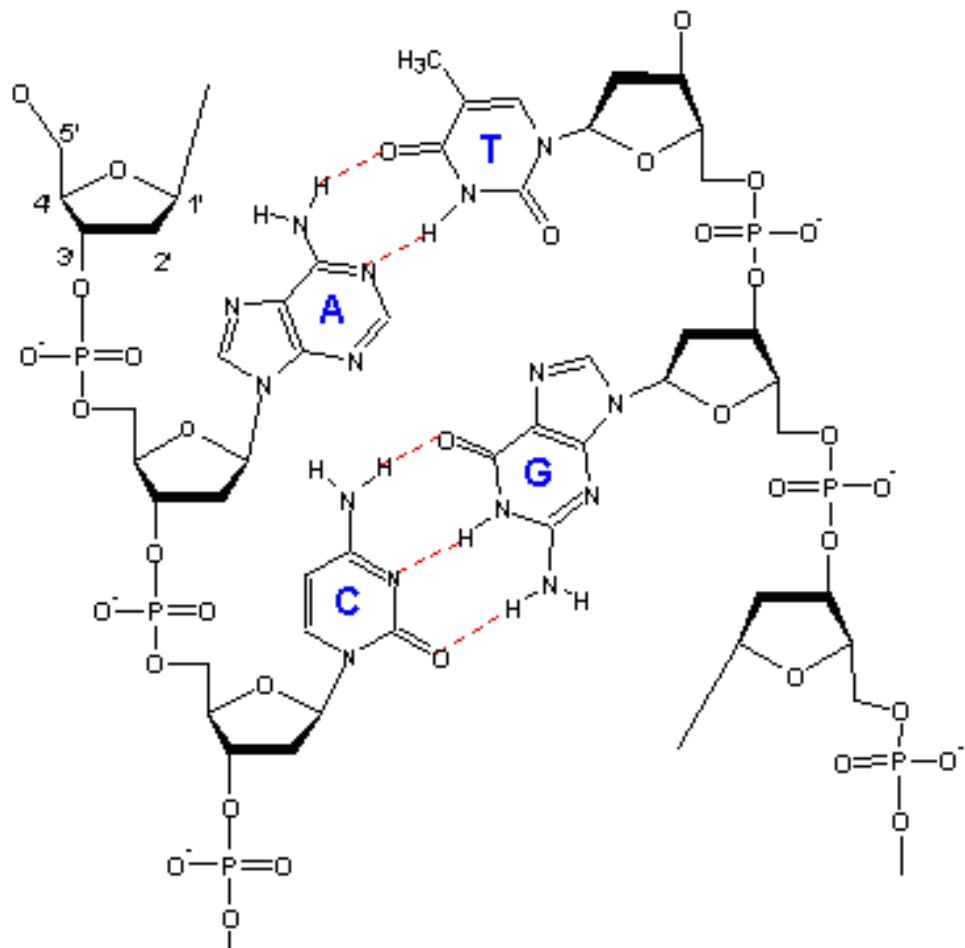
\includegraphics[width=0.65\textwidth]{adn.jpg}

\caption{Structure chimique de l'ADN. Le squelette est composé d'une succession de phosphates et de sucres liés entre eux, chacun des sucres est de plus lié à une base azotée. Les bases azotées peuvent interagir par liaisons hydrogènes et interactions orbitalaires. Les bases s'associent plus facilement avec leur complémentaire (Adénine et Thymine ou Cytosine et Guanine) permettant une certaine variété de structure: repliement d'ADN simple brins ou encore association de deux brins complémentaires formant l'hélice caractéristique de l'ADN dit double brin.(Image emprunter au cours de SERGEI N. SMIRNOV \cite{adnjpeg} }
\label{adn}
\end{center}
\end{figure}

La structure chimique de l'ADN et ses intéractions (rappelées sur la figure \ref{adn}) génèrent des propriétés qui sont fortement dépendantes de la séquence. La diversité des séquences 

Dès la deuxième moitiée des années 70, les premières méthodes de séquençage voient le jours.
\textcolor{red}{mixe à rédiger en combinant les sources wikipédia pour la partie "antique" et un document traitant du séquençage haut débit, besin de demander confirmation à thierry sur certains points avant d'écrire des b\^{e}tises}

\subsubsection{La translocation de polymères}



Très récemment, le développement des expériences sur molécule unique ont permis de s'affranchir des moyennes macroscopiques classiques et d'investiguer en profondeur les processus moléculaires clés en biologie. Il est maintenant possible de manipuler des brins d'ADN notamment en les greffant sur des billes ou des pointes d'AFM \cite{keyser}.\\

\textcolor{red}{ajout d'illustration pour les deux cas}

Ce greffage sur des objets facilement manipulables a permis de déterminer de nombreuses propriétés physique de l'ADN, tel sa résistance ou encore sa longueur de persistance, propriétés qui se révélèrent bien souvent dépendante de la séquence utilisée \textcolor{red}{[réf]}. Parmi les phénomènes dont l'étude est dorénavant possible, figure la translocation. La translocation d'un polymère est son passage par un pore reliant deux compartiments séparés par une membrane.\\

\textcolor{red}{Est ce que j'inclus le paragraphe précédent sur la manipulation d'ADN dans un sous-chapitre en partant d'un peu plus loin avec la chimie de greffage et en mentionnant par exemple que ca sert au creab pour des puces à aptamer ou c'est hors sujet ?}

 Lors de la translocation, la molécule passe d'un coté appelé cis à l'autre appelé trans en deux étapes. La première étape consiste en ce qu'une extrémité de la chaîne atteigne l'entrée du pore. La probabilité d'accéder au pore et le temps caractéristique qui lui est associé ont déjà été estimés analytiquement \cite{milchev}, les outils de manipulations précédemment évoqués permettent le contr\^{o}le  de cette étape. La deuxième étape, qui nous intéresse a lieu lorsque le pore est occupé par le polymère (voir Figure \ref{transloc}). \\

\begin{figure}[H]
\begin{center}
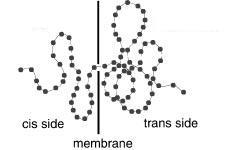
\includegraphics[width=0.45\textwidth]{transloc.jpg}

\caption{Un polymère effectue une translocation d'un coté de la membrane appelé cis vers l'autre appelé trans. Le temps pendant lequel le pore est occupé est appelé temps de translocation (illustration réf: \cite{sung}).}
\label{transloc}
\end{center}
\end{figure}



Le temps pendant lequel le pore est occupé, appelé temps de translocation ($\tau$) est très important puisqu'il représente dans beaucoup de cas la seule mesure expérimentale accessible. Ce temps de translocation va dépendre de plusieurs paramètres notamment la longueur du polymère, l'application éventuelle d'une force (translocation biaisée ou libre), la façon dont elle est appliquée... Nous reviendrons sur ces facteurs dans la partie Aspect théorique.\\

 Une idée directrice des expériences réalisées au cours de la dernière décennie est la mesure du courant ionique à travers le pore au cours de la translocation \cite{holesedge}. Ce courant est caractéristique de l'élément en cours de translocation. Expérimentalement, il a déjà été démontré que la mesure de ce courant de translocation permet de multiples déductions:
 \begin{itemize}
 
 
 
 \item Détecter et identifier des protéines ainsi que leur conformation[\textcolor{red}{réf}].
 
  \item Déterminer la nature de l'ADN (simple ou double brin) ainsi que sa conformation (éventuel repli)[\textcolor{red}{réf}].
  
 \end{itemize}
 
 \textcolor{red}{ajout d'illustration avec variation de courant au cours d'une translocation}
 
Le courant est fortement modifié au cours de ces expériences, cependant la limite de résolution en courant nécessaire afin de séquencer est atteinte. La première source de limitation est temporelle: la translocation a généralement lieu trop rapidement pour que les variations de courant soient observables. La seconde est spatiale. En effet les pores utilisés jusqu'à présent sont bien trop épais et plusieurs dizaines de bases sont simultanément au sein du pore lors de la translocation, ce qui rend très difficile de distinguer les unes des autres les nombreuses séquences possibles.

Les expériences relatives à la translocation d'ADN ont été menées sur toutes sortes de pores, pores que nous allons maintenant présenter.
 
 

\subsubsection{Les nanopores}



\subsubsection*{Les bio-pores:}
Les premiers pores étudiés ont été ceux directement disponibles car existants dans la nature, les bio-pores. Le plus utilisé est l'$\alpha$-hémolysine, il s'agit d'une exotoxine produite par le Staphylocoque doré, c'est ce qu'a utilisé l'équipe de Kasianowicz \cite{kasianowicz} en 1996 en réalisant la première translocation d'ADN. Comme l'illustre la Figure \ref{biopore}, l'ADN peut aisément effectuer une translocation à travers une membrane lipidique par le biais de ce pore. \\

\begin{figure}[H]
\begin{center}
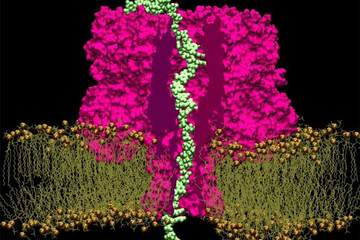
\includegraphics[width=0.45\textwidth]{biopore.jpg}

\caption{Translocation d'ADN grâce à l'$\alpha$-hémolysine, un bio-pore.}
\label{biopore}
\end{center}
\end{figure}

Les bio-pores présentent certains avantages, ils peuvent être cultivés et ont souvent une grande sélectivité vis a vis des molécules autorisées à traverser. Ils permettent ainsi de détecter des protéines ou des ions particuliers. Cependant ils présentent des limitations: leur taille n'est pas modulable, ils nécessitent de travailler en conditions physiologiques. Un des obstacles à leur utilisation pour le séquençage est leur importante épaisseur, comme nous l'avons fait remarquer précédemment.


\subsubsection*{Les pores artificiels de première génération:}

Afin de pallier aux désavantages des bio-pores, des pores artificiels ont été élaborés. Ces pores, principalement basés sur les technologies du silicium, perdent en sélectivité, mais ont des propriétés beaucoup plus adaptables, ce qui permet de quantifier l'influence des paramètres géométriques. A l'instar des bio-pores, leur épaisseur reste trop importante. La Figure \ref{artificialpore} présente un exemple de pore en silice.

\begin{figure}[H]
\begin{center}
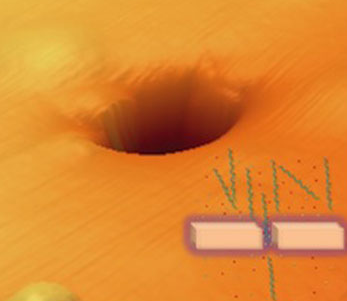
\includegraphics[width=0.3\textwidth]{artificialpore.png} \hspace{0.02\textwidth}
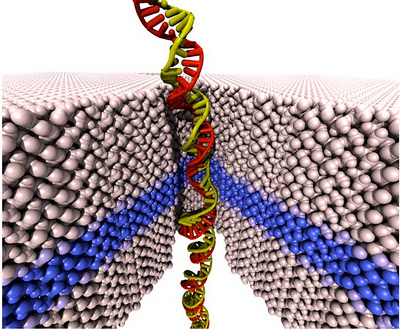
\includegraphics[width=0.35\textwidth]{nanoporeart.jpg}

\caption{Un pore artificiel en silice, imagerie par AFM et modélisation.}
\label{artificialpore}
\end{center}
\end{figure}

Le lecteur intéressé par les possibilités des différents types de pores et l'emploi de divers moyens de contrôles sur la translocation appréciera l'article de revue écrit par Ulrich F. Keyser \cite{keyser}. 




\subsubsection{Les membranes fines}

Comme nous l'avons déjà souligné, le principal obstacle au séquençage par analyse du courant de translocation est l'épaisseur trop importante du pore qui ne permet pas de distinguer les multiples combinaisons de séquences possibles. Ce problème pourrait bien être résolu par l'utilisation de membranes très fines dont le graphène fait partie.\\

Isolé pour la première fois en 2004, le graphène est un cristal bidimensionnel de carbone \cite{graph}. L'empilement de plusieurs couches monoatomiques de graphène forme le graphite. Comme le montre la Figure \ref{orbit}, les carbones forment un maillage hexagonal de paramètre de maille d= 0.142 $nm$, les électrons délocalisés sur l'ensemble des orbitales $\pi$ de ce plan le rendent aromatique. L'occupation de ces orbitales $\pi$ est l'origine de propriétés intéressantes du graphène. Les électrons $\pi$ octroient au graphène une importante conductivité. Les interactions orbitalaires (stacking) maintiennent une cohésion entre les différents plans. La distance inter-planaire dans le graphite, 0.335 $nm$, est plus importante que la distance inter-atomique dans le plan, cela est dû à la géométrie plus étendue perpendiculairement au plan des orbitales $\pi$.

\begin{figure}[H]
\begin{center}
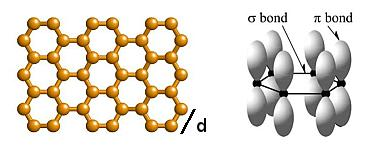
\includegraphics[width=0.57\textwidth]{orbitals2.jpg} 
\caption{Structure cristallographique et orbitales $\pi$ du graphène.}
\label{orbit}
\end{center}
\end{figure}
 
Expérimentalement, il a été vérifié que la translocation d'ADN à travers un nanopore creusé dans le graphène est possible \cite{dnatrans}. C'est une porte ouverte à de nombreuses autres expériences. La finesse de la couche monoatomique de graphène entraîne cependant des différences singulières par rapport aux pores utilisés précédemment. En effet, l'épaisseur importante d'un pore impose une certaine rigidité à ce dernier. Ce n'est plus le cas lors de l'utilisation de pores creusés dans le plan de graphène, qui est déformable et présente des propriétés vibrationnelles complexes, comme l'illustre la Figure \ref{vib}.


\begin{figure}[H]
\begin{center}
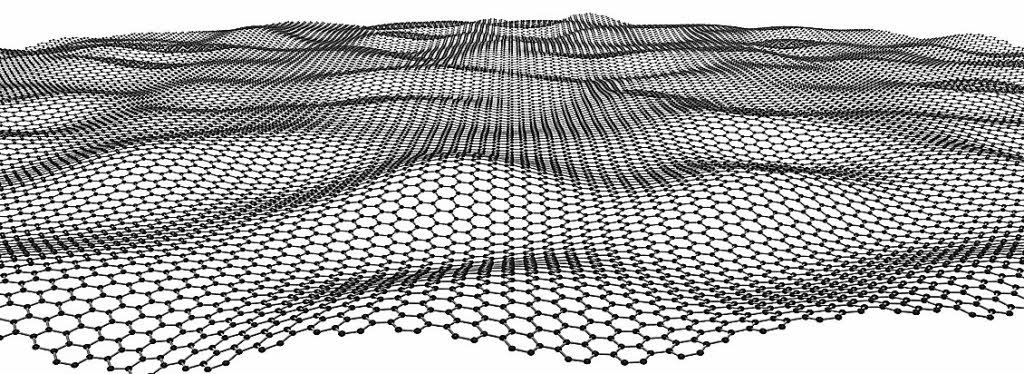
\includegraphics[width=0.83\textwidth]{vib.jpg} 
\caption{La couche monoatomique de graphène, flexible, présente des propriétés vibrationnelles complexes.}
\label{vib}
\end{center}
\end{figure}

D'autre cristaux bidimensionels sont depuis peu également disponibles, tel le *** [\textcolor{red}{réf}]. Ces nouvelles conditions expérimentales n'ont pour l'instant pas de cadre général théorique pour leur étude.\\

La prochaine section explicite le cadre analytique disponible pour l'étude de la translocation et montre quelles sont ses limites vis a vis des conditions  envisagées.


\newpage

\subsection{Aspect théorique}


\subsubsection{Polymères idéaux et non idéaux}
Nous allons dans un premier temps présenter un modèle naïf de polymère idéal afin de poser les bases admises en physique des polymères \cite{sung,these}.\\

Le polymère évolue sur un réseau périodique de paramètre $\lambda$. La tête du polymère est placée sur un des nœuds du réseau. Les monomères consécutifs sont placés sur un des $z$ ($z=4$ pour un réseau carré) sites plus proches voisins, le polymère réalise alors une marche aléatoire (Figure \ref{resideal}).

\begin{figure}[H]
\begin{center}
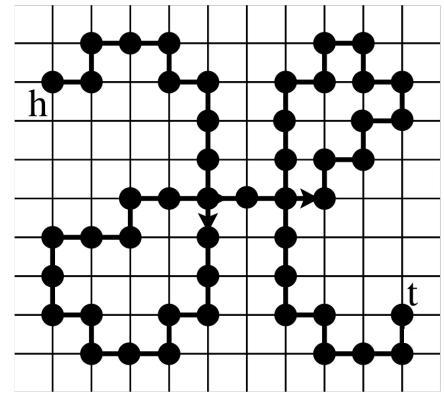
\includegraphics[width=0.35\textwidth]{resideal.jpg}

\caption{Réseau carré montrant la marche aléatoire qui génère une configuration d'un polymère \cite{these}.}
\label{resideal}
\end{center}
\end{figure}

On déduit facilement que pour un degré de polymérisation $N+1$, il y a $Z_{ideal}=z^N$ polymères distincts possibles. Recalculons les résultats fondamentaux concernant la marche aléatoire génératrice du polymère (ces résultats sont indépendants du réseau qui est un artifice de calcul et ne modifie pas les lois d'échelle, la pluspart des modèles numériques n'utilisent pas de maillage). Soit $\textbf{r}$ le vecteur position du marcheur par rapport à l'origine et $b$ la taille d'un pas effectué par le marcheur. Soit $\textbf{r}_n$ le $n$-ième pas effectué, au bout d'un nombre de pas $N$, on a: 

\begin{eqnarray}
\textbf{r} = \sum_{n = 1}^{N} \textbf{r}_n
\end{eqnarray}

Pour la marche aléatoire idéale, il n'y a pas de corrélation entre les différents pas, ce qui mathématiquement se traduit par $\left<\textbf{r}_i \cdot \textbf{r}_j\right> = \delta_{i,j} b^2$. Ce qui implique les relations suivantes:

\begin{eqnarray}
\left<\textbf{r}\right>\text{} = \sum_{n = 1}^{N} \left<\textbf{r}_n \right>\text{} =\text{} 0 \text{ }, \text{} \left<\textbf{r}^2\right> \text{}= \sum_{i = 1}^{N} \sum_{j = 1}^{N} \left<\textbf{r}_i \cdot \textbf{r}_j\right> \text{}= \sum_{i = 1}^{N} \left<\textbf{r}_i^2\right> \text{}= b^2 N
\label{rdmwalk}
\end{eqnarray}

 Puisque la valeur moyenne de $\textbf{r}$ est nulle, on estime le comportement de la distance entre les extrémités (distance end-to-end) moyenne du polymère en prenant la racine carré de la valeur moyenne de $\textbf{r}^2$. Comme le montre l'équation \ref{rdmwalk} la distance end-to-end du polymère sera proportionnelle à $N^\frac{1}{2}$.\\
 
 Une estimation correcte de la taille du polymère est obtenue en considérant le rayon de giration $R_g$. Il est défini de la manière suivante en notant $\textbf{r}_{CM}$ la position du centre de masse du polymère :
 \begin{eqnarray}
R_g^2\text{}=\text{}\frac{1}{N}\sum_{n = 1}^{N} \left<(\textbf{r}_n-\textbf{r}_{CM})^2\right>
 \text{ ou encore, de manière équivalente: }
R_g^2\text{}=\text{}\frac{1}{2N^2}\sum_{i,j}^N \left<(\textbf{r}_i-\textbf{r}_{j})^2\right>
\label{equ}
\end{eqnarray}
 
 L'équivalence s'obtient en développant les termes des deux expressions et en les identifiant.\\


On va appliquer la dernière partie de l'équation \ref{rdmwalk} pour la marche aléatoire à l'équation \ref{equ} du rayon de giration en notant le fait qu'on effectue une marche aléatoire de $|i-j|$ pas pour aller du monomère $i$ au $j$ dans l'expression $\left<(\textbf{r}_i - \textbf{r}_j)^2\right>$.

\begin{gather}
R_g^2\text{}=\text{}\frac{1}{2N^2}\sum_{[|i-j|]} |i-j| b^2=\text{}\frac{1}{N^2}\sum_{[i>j]} |i-j| b^2\nonumber \\
=\text{}\frac{b^2}{N^2} \sum_{i=1}^N \sum_{j=1}^{i} j \\
 = \text{}\frac{b^2}{N^2}[\frac{1}{2}(\frac{N(N+1)(2N+1)}{6}+\frac{N(N+1)}{2})]\nonumber
\label{gyr}
\end{gather}

En prenant la limite $N \gg 1$ dans l'équation précédente (\ref{gyr}), on obtient la loi d'échelle à laquelle le rayon de giration obéit:
\begin{eqnarray}
R_g^2\text{}\sim\text{}\frac{b^2}{6}N \Rightarrow R_g\propto N^{\frac12}
\end{eqnarray}

La distance end-to-end et le rayon de giration obéissent à la même loi d'échelle et sont caractéristiques de l'expansion spatiale du polymère.\\


Revenons à notre modèle sur réseau afin d'établir une équation différentielle sur la probabilité, $P(\textbf{r},N)$, du $N$-ième monomère d'être en $\textbf{r}$. Pour cela, introduisons les z $\textbf{b}_i$  vecteurs les plus proches de la position $\textbf{r}$ pour obtenir:
\begin{eqnarray}
P(\textbf{r},N)= \frac{1}{z}\sum_{i=1}^{z} \left[P(\textbf{r}-\textbf{b}_i,N-1)\right]
\label{eqdifprob}
\end{eqnarray}

On effectue ensuite un développement limité à l'ordre 2 afin d'obtenir une équation différentielle à résoudre sur la probabilité de distribution. On fait comme hypothèse que $\textbf{r}>>\textbf{b}_i$ et $N >> 1$.

\begin{eqnarray}
P(\textbf{r}-\textbf{b}_i,N-1)=P(\textbf{r},N)- \frac{\partial P}{\partial N}-  \textbf{b}_{i\alpha} \frac{\partial P}{\partial r_{\alpha} } + \frac12 \textbf{b}_{i\alpha}\textbf{b}_{i\beta} \frac{\partial ^2 P}{\partial r_{\alpha}\partial r_{\beta} }
\end{eqnarray}

En utilisant la convention de sommation d'Einstein, $i$ varie de $1$ à $z$ et $\alpha$ et $\beta$ représentent les coordonnées spatiales. En considérant les résultats suivants:

\begin{eqnarray}
\sum_{i=1}^{z}\textbf{b}_{i\alpha}=0 \text{ },\text{ } \sum_{i=1}^{z}\textbf{b}_{i\alpha}\cdot\textbf{b}_{i\beta} = \frac{b^2\delta_{\alpha,\beta}}{3}
\end{eqnarray}

On obtient l'équation différentielle qui régit la probabilité de distribution de nos monomères:
\begin{eqnarray}
 \frac{\partial P}{\partial N} =   \frac{b^2}{6}\frac{\partial ^2 P}{\partial ^2 \textbf{r}}
 \label{eqdif}
\end{eqnarray}

Cette équation différentielle (\ref{eqdif}) a pour solution avec pour condition initiale $\textbf{r}=0$ quand $N=0$ :
\begin{eqnarray}
P(\textbf{r},N)=\left(\frac{3}{2\pi N b^2}\right)^\frac{3}{2}\exp\left(-\frac{3\textbf{r}^2}{2 N b^2}\right)
\end{eqnarray}

La distribution de probabilité de présence des monomères est donc gaussienne, un polymère idéal est d'ailleurs souvent dit gaussien.\\

Remarquons dors et déjà que le logarithme de la distribution de probabilité donne par définition l'énergie libre du système qui n'est pas sans rappeler celle d'un ressort:
\begin{eqnarray}
F(\textbf{r})= - k_B T \ln(P(\textbf{r},N))= F(0)+\frac{3k_BTr^2}{2Nb^2}
\label{elibre}
\end{eqnarray}
$k_B$ est la constante de Boltzmann. Cette énergie sera utilisée par la suite pour décrire des propriétés dynamiques du polymère.\\



Bien entendu ce modèle est simpliste, un vrai polymère ne peut en aucun s'intersecter lui même, les monomères peuvent être différents, il peut ne pas être linéaire...\\

 Traitons le cas d'un polymère qui ne peut s'intersecter lui-même. Les configurations sont alors générées par des marches aléatoires auto-évitantes (Self Avoiding Walks ou SAW). Soit $v_c \propto b^3$ le volume exclusif occupé par un monomère. La probabilité qu'un monomère de la chaîne de volume $R^3$ ne se superpose pas à un autre est $(1-\frac{v_c}{R^3})$, il y a $\frac{N(N-1)}{2}$ paires de monomères. La probabilité totale de non superposition est donc:
 \begin{eqnarray}
P_{ns}(N)= \left(1-\frac{v_c}{R^3}\right)^{\frac{N(N-1)}{2}} = \exp\left[\frac{N(N-1)}{2}\text{ }\ln\left(1-\frac{v_c}{R^3}\right)\right]
\end{eqnarray}

La probabilité de distribution d'une SAW est donc le produit des deux probabilités précédentes, ce qui donne dans la limite $N \gg 1$, $R \gg v_c$:
\begin{eqnarray}
P_{SAW}(R,N)=P_{ns}(N) P(R,N)=\exp\left[-\frac{3R^2}{2 N b^2}-\frac{v_cN^2}{2R^3}\right]
\end{eqnarray}

La taille caractéristique du polymère est alors donnée par la valeur $R^*$ qui maximise la probabilité de distribution, d'où:

\begin{gather}
\frac{\partial P_{SAW}(R,N)}{\partial R} \Huge{|} _{R=R^*}=0 \nonumber\\
\Rightarrow \frac{3R^{*2}}{Nb^2}-\frac{3v_cN}{2R^{*4}} =0 \\
\Rightarrow R^* \propto N^\frac{3}{5}\nonumber
\end{gather}


La taille caractéristique du polymère croit donc plus rapidement avec le nombre de monomères que dans le cas idéal précédent. L'exposant 3/5 trouvé est très proche de l'exposant de Flory, $\nu=0.588$, qui fait consensus (réf) parmi les différentes simulations numériques. \\


Le cas de la chaîne auto évitante est adapté aux polymères dilués en solution. Le modèle de la chaîne idéale décrit paradoxalement très bien un contexte de polymères en forte concentration en contacte les uns des autres. En effet les termes de volumes exclus s'appliquent pour le polymère aussi bien par sa propre chaîne que par la présence de chaînes voisines. L'espace précédemment libre est occupé, le volume exclu apporte une contribution énergétique uniforme dans tout l'espace. Les termes de volumes exclus se compensent donc tous, ce qui permet de se retrouver uniquement avec la contribution d'une chaîne idéale.

\subsubsection{Dynamique des polymères}

Nous allons maintenant proposer un modèle permettant d'aborder la dynamique d'une chaîne. Il s'agit du modèle de Rouse (Figure \ref{rouse}). Comme nous l'avions signalé, l'énergie libre d'un polymère idéal présente les caractéristiques d'un potentiel harmonique de type ressort (cf: équation \ref{elibre}), ce qui justifie cette modélisation.

\begin{figure}[H]
\begin{center}
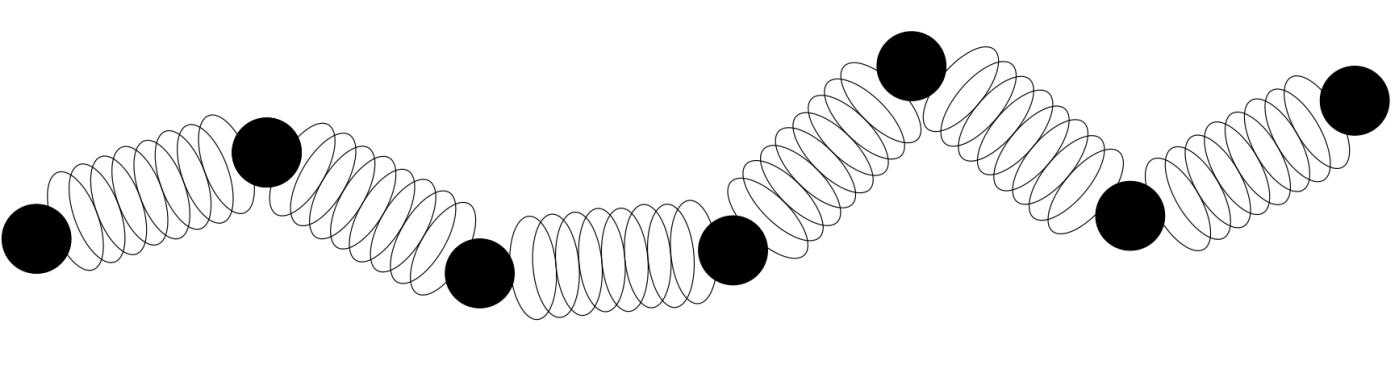
\includegraphics[width=0.65\textwidth]{rouse.jpg}

\caption{Modélisation du polymère par une chaîne d'oscillateurs.}
\label{rouse}
\end{center}
\end{figure}

Le polymère est modélisé par une chaîne d'oscillateurs (de type billes/ressorts). Physiquement, le ressort ne représente pas une liaison entre monomères mais plutôt une partie du polymère assez longue pour que la statistique gaussienne puisse lui être appliquée. De l'équation \ref{elibre} obtenue précédemment on déduit l'énergie élastique du ressort connectant les billes $n$ et $n+1$ séparées par une distance d'équilibre moyenne $b$:


\begin{eqnarray}
F_{n,n+1} = \frac{3 k_B T}{2} \frac{(\textbf{r}_{n+1}-\textbf{r}_n)^2}{b^2}
\end{eqnarray}

Nous nous plaçons dans des conditions simples en modélisant l'effet du solvant par un simple terme de frottement visqueux (ou Stokes drag), la trajectoire est donc donnée par l'équation de Langevin \ref{langevin} qui s'écrit ici:

\begin{eqnarray}
\large{
\frac{d \textbf{r}_n}{dt} =  \frac{3T}{\nu_n b^2}( \textbf{r}_{n+1} +\textbf{r}_{n-1} -2\textbf{r}_n )  + \textbf{g}_n}
\end{eqnarray}

On va résoudre cette équation en prenant $n$ comme variable continue.

\begin{eqnarray}
\large{
\frac{d \textbf{r}}{dt} =  \frac{3T}{\nu b^2}\frac{\partial ^2 \textbf{r}}{\partial  n^2} + \textbf{g}_n}
\end{eqnarray}

Avec les conditions limites $\frac{\partial  \textbf{r}}{\partial  n}=0$ en bouts de chaine, on peut résoudre le système en le séparant en plusieurs modes à  partir de coordonnées normalisées: 
\begin{eqnarray}
\textbf{x}_p= \frac{1}{N} \int_0^N \cos \left(\frac{n\pi p}{N}\right) \text{ }\textbf{r}(n,t)\text{ } dn \text{ , } \frac{d \textbf{x}_p}{dt} =  -\frac{k_p}{\nu _p} \textbf{x}_p + \textbf{g}_p
\end{eqnarray}



\begin{eqnarray}
\nu_0=  N \nu \text{ , } \nu_p= 2 N \nu  \text{ , }  k_p=\frac{6T\pi^2 p^2}{N b^2}  \text{ , }  \left<\textbf{g}_{p\alpha}(t) \cdot \textbf{g}_{q\beta}(t')\right> = 2\delta_{p,q} \delta_{\alpha ,\beta} \frac{T}{\nu_p} \delta(t-t')
\end{eqnarray}

En travaillant dans la nouvelle base orthogonale, on peut montrer que:


\begin{eqnarray}
\left<(\textbf{x}_{0}(t)-\textbf{x}_{0}(0))_\alpha \cdot (\textbf{x}_{0}(t)-\textbf{x}_{0}(0))_\beta \right> = 2 \delta_{\alpha ,\beta} \frac{T}{N\nu}t
\end{eqnarray}

\begin{eqnarray}
\left<\textbf{x}_{p\alpha}(t) \cdot \textbf{x}_{q\beta}(0)\right> = 2\delta_{p,q} \delta_{\alpha ,\beta} \frac{T}{k_p} \exp\left(-\frac{t}{\tau_p}\right) \text{ , } \tau _p = \frac{\nu N^2 b^2}{3\pi^2p^2T}
\end{eqnarray}

La distance end-to-end et le rayon de giration sont des combinaisons linéaires des $\textbf{x}_p$ et sont donc assujettis  au temps de relaxation le plus long, $\tau_1$ qui obéit à la loi d'échelle : $\tau_1 \propto N^2$. De même la position du centre de masse est donnée par $\textbf{x}_0$, ce qui permet d'en déduire le coefficient de diffusion du polymère:


\begin{eqnarray}
\left<(\textbf{r}_{CM}(t)-\textbf{r}_{CM}(0))^2\right>=\frac{6 k_B T}{N \nu} t = 6 D_R t
\label{fluctudissip}
\end{eqnarray}




L'équation précédente (\ref{fluctudissip}) traduit le théorème de fluctuation dissipation  en prenant en compte $N \nu$, le coefficient de Stokes global du polymère. Le temps de relaxation peut également être vu comme le temps mis par le centre de masse pour parcourir sa longueur.

 Le temps nécessaire au parcours d'une certaine distance est indépendant de la présence d'intéractions entre monomères (chaîne idéale ou SAW), mais la longueur du polymère dépend des conditions du modèle. On a alors $\tau \propto \frac{R_0^2}{D}$, soit $\tau \propto N^2 $ dans le cas idéal ou $\tau \propto N^{1+2\nu} $ dans le cas de la marche auto-évitante. 

Expérimentalement, on ne retrouve pas ces résultats car le modèle néglige les intéraction hydrodynamiques, des intéractions à longue portée entre les monomères via le solvant. La figure \ref{hydrodyninterac} illustre ce phénomène.


\begin{figure}[H]
\begin{center}
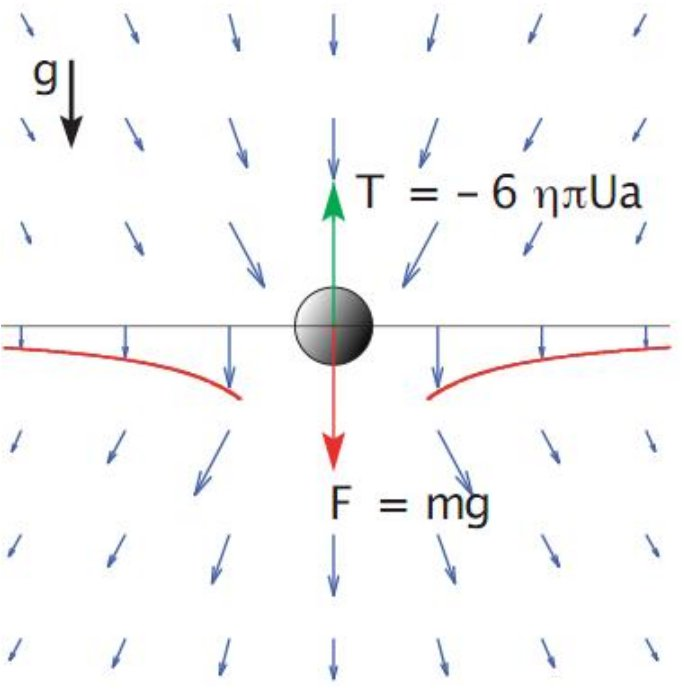
\includegraphics[width=0.4\textwidth]{hydrodyninterac.jpg} 

\caption{Mouvement de fluide généré par une bille en chute libre. Pour chaque objet en mouvement, Le fluide déplacé génère un champ de vitesse, ces champs de vitesse décroissent en l'inverse de la distance et se superposent.}
\label{hydrodyninterac}
\end{center}
\end{figure}

La compréhension de la dynamique des polymères permet de s'attaquer à l'élaboration de modèles pour la translocation.










\subsubsection{Translocation}



La translocation peut se dérouler dans différents contextes. Elle peut être due uniquement aux fluctuations thermiques, on parle alors de translocation non biaisée, ou être pilotée par une force extérieure, on parle alors de translocation forcée (driven translocation). Les forces extérieures peuvent être de natures variées, on citera notamment l'utilisation de champs électriques (électrophorèse), de gradients de potentiels chimiques, de flux imposé sur le solvant, ou encore l'emploi de pinces optiques \cite{keyser}.\\

Le temps de translocation dépend alors fortement de la taille du polymère et de la force appliquée, d'une façon générale on peut définir des lois d'échelles:

\begin{eqnarray}
\tau = N^\alpha f^{-\delta}
\label{tau}
\end{eqnarray}

 Le but du stage est de déterminer les valeurs de $\alpha$ et $\delta$, appelés exposants critiques, dans les différentes limites possibles. On basera l'échelle de force en unités de Lennard-Jones à partir de la valeur de $\frac{\epsilon}{b}$.\\

Nous allons dans un premier temps calculer la forme de la barrière d'énergie franchie par le polymère lors de la translocation. Pour cela, nous devons dans un premier temps calculer la probabilité de distribution d'un polymère idéal greffé à une paroi. La chaîne idéale présente comme conditions aux limites, la non pénétration des monomères à travers la paroi. On note $P(\textbf{r},\textbf{r}_0,n)$ la probabilité de trouver le $n$-ième monomère en position $\textbf{r}$, pour $n \gg 1$, le premier monomère étant greffé en $\textbf{r}_0$. $P_0$ est la distribution calculé précédemment pour un polymère idéal libre.

\begin{eqnarray}
P_0(\textbf{r},\textbf{r}_0,n)=\left(\frac{3}{2\pi n b^2}\right)^\frac{3}{2}\exp\left(-\frac{3(\textbf{r}-\textbf{r}_0)^2}{2 n b^2}\right)
\end{eqnarray}

A l'instar de nombreux problèmes d'électromagnétisme ou de mécanique des fluides, on utilise la méthode des images miroirs afin de déterminer $P(\textbf{r},\textbf{r}_0,n)$. En effet, on a:

\begin{eqnarray}
P(\textbf{r},\textbf{r}_0,n) \propto P_0(\textbf{r},\textbf{r}_0,n)-P_0(\textbf{r},-\textbf{r}_0,n)
\end{eqnarray}

Dans le cas idéal, la probabilité de distribution du monomère de queue est à variables séparables. En posant $\textbf{r}_0= \epsilon y$ avec $\epsilon \ll 1$, un développement limité au premier ordre donne:

\begin{eqnarray}
P(\textbf{r},\textbf{r}_0,n) \propto \left(\frac{3}{2\pi n b^2}\right)^\frac{3}{2} \left(\frac{6 y \epsilon}{n b^2}\right)\exp\left(-\frac{3\textbf{r}^2}{2 n b^2}\right)
\end{eqnarray}

Pour le cas non idéal, les termes supplémentaires introduits dans $P_0$ ne permettent pas de séparer les variables et d'obtenir une expression analytique.


\begin{figure}[H]
\begin{minipage}{0.45\linewidth}
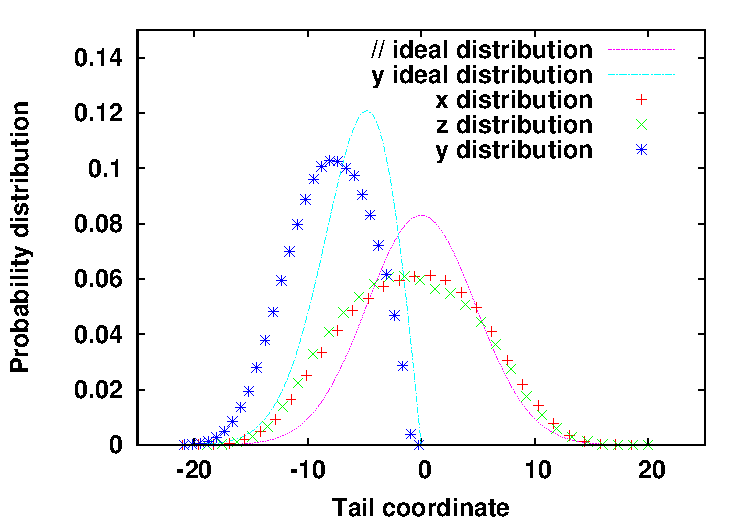
\includegraphics[width=1.2\textwidth]{probdistribution.pdf}

\end{minipage}\hfill
\begin{minipage}{0.45\linewidth}
\caption{Probabilité de distribution théorique du monomère de queue pour un polymère idéal et résultats numériques pour un polymère à monomères durs (N=35). Parallèlement à la membrane, la distribution gaussienne idéale est aplatie au centre à cause de la zone d'exclusion des autres monomères. De même pour la direction perpendiculaire, le pic maximum est repoussé par la présence d'autres monomères. Dans les deux cas, l'éloignement maximal n'est pas modifié car le cas idéal correspond déjà à des chaînes étirées sans superpositions de monomères. }
\label{polagainstwall}
\end{minipage}
\end{figure}


Afin d'aborder la translocation, nous avons du créer des configurations indépendantes de polymères à l'équilibre, juste avant l'application d'une force. Lors de ce processus de génération, nous avons laisser le polymère évoluer librement en fixant une extrémité au centre du pore. L'étude des coordonnées du grain de queue nous a permis d'évaluer l'influence des volumes exclus, comme le montre la Figure \ref{polagainstwall}.


La probabilité de distribution du polymère accolé à une membrane permet, à partir de la fonction de partition stérique, $Z_S(n)= \int_{y>0} P(\textbf{r},\textbf{r}_0,n) \textbf{dr}$, de calculer l'énergie libre d'origine entropique d'un tel système. Dans la limite $n \gg 1$, le premier terme non nul du développement limité impose la loi d'échelle: $Z_S(n) \propto n^{-1/2}$. Pour un polymère de $N$ monomères en cours de translocation, lors du passage du $n$-ième monomère, on obtient la valeur de l'énergie libre en prenant en compte les effets entropiques de part et d'autre de la membrane:
\begin{eqnarray}
F(N,n)= -k_BT\ln\left(Z_S(n)Z_S(N-n)\right)= \frac{1}{2} k_BT \ln \left(n(N-n)\right) +cste
\end{eqnarray}

Cette barrière d'énergie à franchir au cours de la translocation peut être altérée en appliquant une différence de potentiel, chimique ou électrique, ou encore en appliquant directement une force sur la chaîne. La Figure \ref{energiebarrier} montre cette barrière d'énergie.
\begin{figure}[H]
\begin{center}
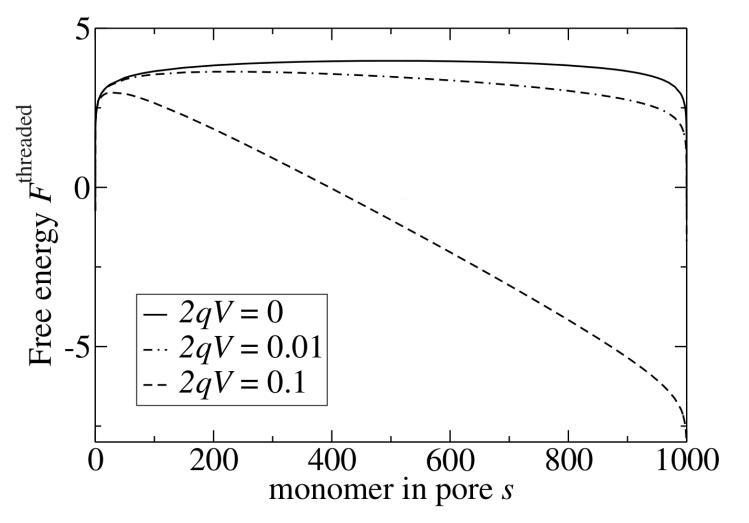
\includegraphics[width=0.4\textwidth]{transelec.jpg} 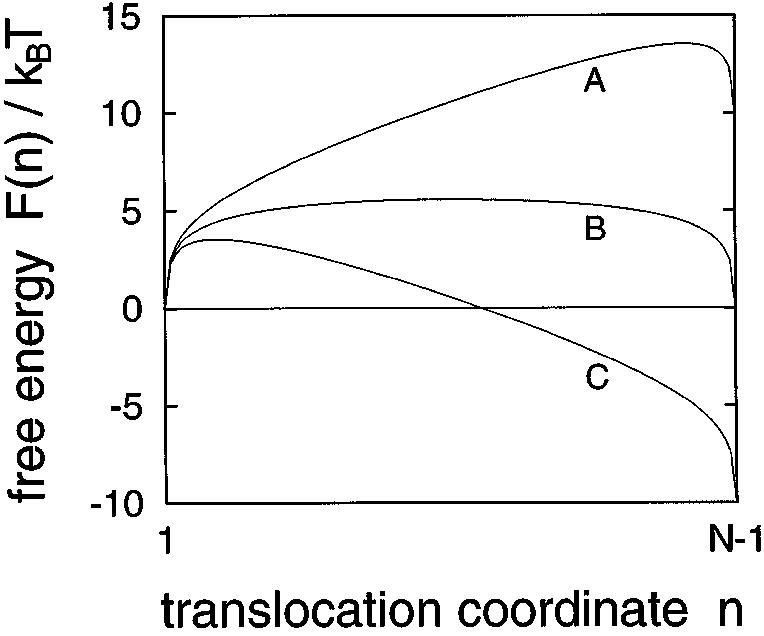
\includegraphics[width=0.28\textwidth]{transpotchim.jpg}

\caption{Modification de la barrière entropique par une différence de potentiel électrique (à gauche \cite{these}) et de potentiel chimique (à droite \cite{sung}). A: différence de potentiel opposée à la translocation, B: différence de potentiel nulle, C: différence de potentiel favorable.}
\label{energiebarrier}
\end{center}
\end{figure}

 Lors de la translocation non biaisée, la barrière d'énergie est utilisée pour résoudre l'équation de Smoluchowski, qui va permettre de déduire $\tau \propto N^{1+2\nu}$ comme limite inférieure. Le cas non biaisé n'a pas été étudié. Le lecteur intéressé trouvera démonstrations et explications dans l'article de revue de Milchev \cite{milchev}.
 
 Pour la translocation forcée, l'application d'une force bouleverse l'hypothèse de l'équilibre thermodynamique local utilisée pour évaluer $\tau$ dans le cas non biaisé. Plusieurs modèles hors équilibre sont présentés dans l'article de J. L. A. Dubbeldam et collaborateurs \cite{traction}. Nous retenons de la lecture de cet article que pour la dépendance en $N$, ils s'attendent à une transition de $\tau \propto N^{2\nu}$ à $\tau \propto N^{1+\nu}$ lorsque la force augmente. En ce qui concerne la dépendance en $F$, ils s'attendent à une transition de $\tau \propto F^{-1}$ à $\tau \propto F^{(1/\nu)-2}$ lorsque la taille de la chaîne diminue.



\subsubsection*{Translocation à travers un pore large}

Dans un premier temps, nous avons considéré une membrane fixe munie d'un nanopore large. Le nanopore est créé en supprimant 54 grains au centre. L'extrémité du polymère est alors tirée par l'ajout d'une force perpendiculaire à la membrane et d'amplitude modulée sur 3 ordres de grandeurs, de 0.1 à 100. Un cylindre de sécurité est implanté dans le code pour vérifier que le pore est toujours peuplé. Lorsque ce n'est plus le cas, nous vérifions si le polymère a terminé sa course du coté cis ou du coté trans. En effet, pour de faibles forces, le polymère peut dans certaines simulations, ne pas effectuer la translocation.\\

Trois polymères ont été étudiés, ils présentent 8, 16 et 32 monomères. A l'instar des prédictions de J. L. A. Dubbeldam et collaborateurs \cite{traction}, nous observons deux régimes distincts caractérisant la dépendance de la loi d'échelle avec la force. En effet, on observe à forces faibles (excepté pour $N=8$) et intermédiaires un comportement tel que $\tau \propto 1/F$. Pour des forces plus élevées, on trouve une loi d'échelle avec un exposant plus élevé ($\tau \propto F^{-0.74}$ pour N=8) Cet exposant plus élevé montre la transition vers $\tau \propto F^{(1/\nu) -2}$. La valeur plus faible qu'attendue peut être attribuée aux effets de taille finie et à l'amplitude de la force qui n'est pas assez élevée. De plus la transition entre les régime semble apparaitre plus tôt pour les $N$ faibles, contrairement à la prédiction de J. L. A. Dubbeldam et collaborateurs \cite{traction}. Cette différence pourrait venir du fait que nous tractons notre polymère (force en bout de chaîne), alors que dans leur cas, une différence de potentiel est appliquée (force au sein du pore). La Figure \ref{holebigger} permet de mieux visualiser ces régimes. En ce qui concerne l'évolution de $\tau$ avec $N$, on trouve un exposant de 1.78 pour les forces imposées de 9 et 20, et 1.69 pour 80. Ces valeurs sont proches du cas $\tau \propto N^{(1+\nu)}$ attendu pour les forces importantes.

Dans le cas $N=8$, nous observons un décrochement de pente. Ceci se produit lorsque la force est faible et pour une chaîne très courte. L'impulsion initiale donnée par le mouvement brownien rejette nombre de configurations (d’où une forte diminution du nombre de translocation réussies), celles conservées ayant une grande impulsion non naturelle dans le sens de la translocation, diminuant artificiellement $\tau$. Cette rupture de pente nous semble donc être un effet de taille finie.

Exercer des forces plus faibles nous ferait perdre beaucoup trop d'événements. Afin de balayer de larges domaines, il pourrait être intéressant de travailler, comme cela peut être fait expérimentalement à vitesse de traction imposée (la force n'est alors plus constante).

\begin{figure}[H]
\begin{center}
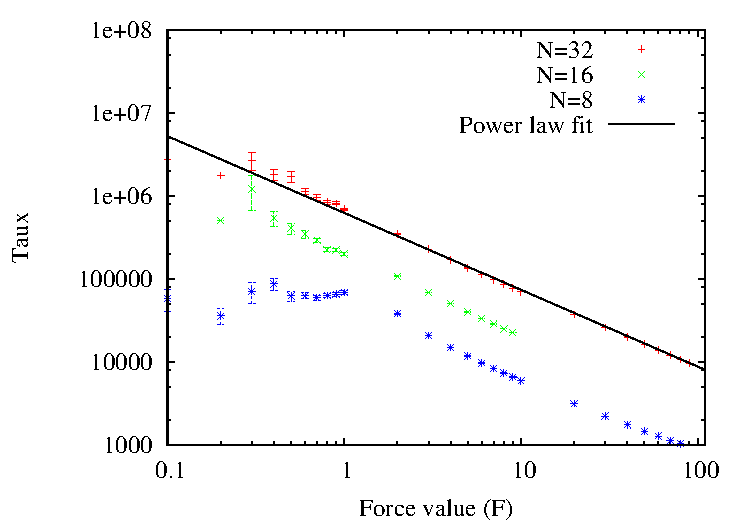
\includegraphics[width=0.48\textwidth]{translocfholebigger.pdf} 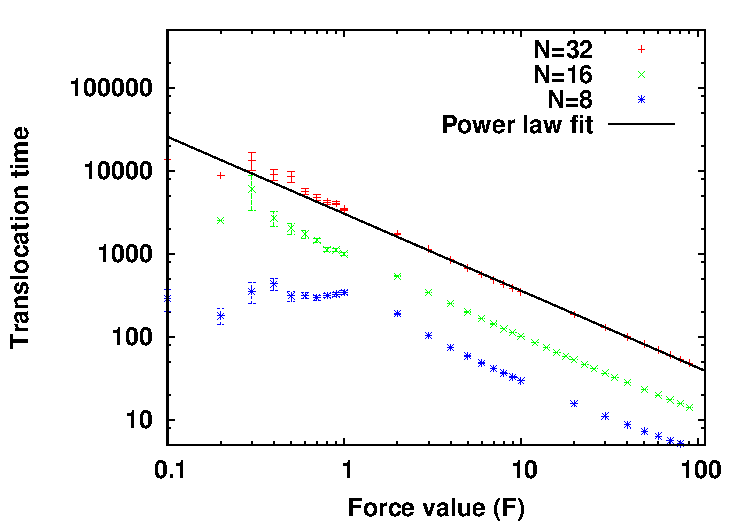
\includegraphics[width=0.48\textwidth]{translocholebigger.pdf}

\caption{Lors de la translocation à travers un pore large, on distingue deux régimes, une décroissance de $\tau \propto 1/F$ suivit d'une augmentation de l'exposant critique quand $F$ devient suffisamment grande. La rupture de pente du cas $N=8$ est imputée à des effets de taille finie. On trouve bien des valeurs proches de $\tau \propto N^{1+\nu}$ pour la dépendance en N.}
\label{holebigger}
\end{center}
\end{figure}

Afin de ralentir la translocation, enjeu clé du séquençage, nous allons maintenant étudier l'influence d'un nanopore plus étroit. En quoi le frottement important induit par le pore va-t-il modifier les lois d'échelle trouvées précédemment?


\subsubsection*{Translocation à travers un pore étroit}
Nous étudions dorénavant l'effet d'une membrane fixe munie d'un nanopore étroit qui va induire un frottement plus important. Le nanopore est créé en supprimant uniquement 24 grains au centre cette fois ci. Le pore a été choisi suffisamment étroit pour empêcher les monomères de passer de front, ils devront se déformer pour permettre le passage du grain latéral, plus volumineux.\\

Encore une fois, nous observons les deux régimes précédents. Cependant la frontière semble apparaitre plus tard à cause du frottement, ce qui diminue la force effective appliquée sur le polymère ($F_{eff}=F-\epsilon _{pore})$. Les mêmes lois d'échelles sont observées à forte force ( $\tau \propto 1/F$ puis $\tau \propto F^{(1/\nu) -2}$).\\

 Une grande différence s'observe dans le cas de l'application de forces faibles. Comme la Figure \ref{thinpore} le suggère, les translocations n'ont pas pu être menées à bien pour des forces inférieures à l'unité.

Les contraintes stériques choisies entrainent une modification de la barrière d'énergie. La translocation des grains par groupe de trois (1 grain latéral volumineux à la fois), comme nous l'illustrerons dans la section suivante (Figure \ref{temperature}), corrobore une hypothèse de déformation de la barrière entropique en dents de scies décroissante. Cette modification est significative puisqu'elle empêche complétement la translocation si la force appliquée est trop faible, elle semble aussi être responsable du comportement inattendu décrit dans la Figure \ref{thinpore}.

Le cas $N=8$ présente encore une fois des problèmes. Lorsque la force est trop faible, les polymères ne pénètrent pas à travers la membrane. Dans le cas de $N=8$, la force est à peine suffisante pour permettre la translocation et n'est pas prépondérente par rapport au bruit thermique. Le polymère passe alors un temps important à rebondir sur le pore avant d'entamer la translocation. Le temps de translocation est alors fortement surévalué (un point a été conservé sur la Figure \ref{thinpore}, pour illustrer ce problème).



\begin{figure}[H]
\begin{center}
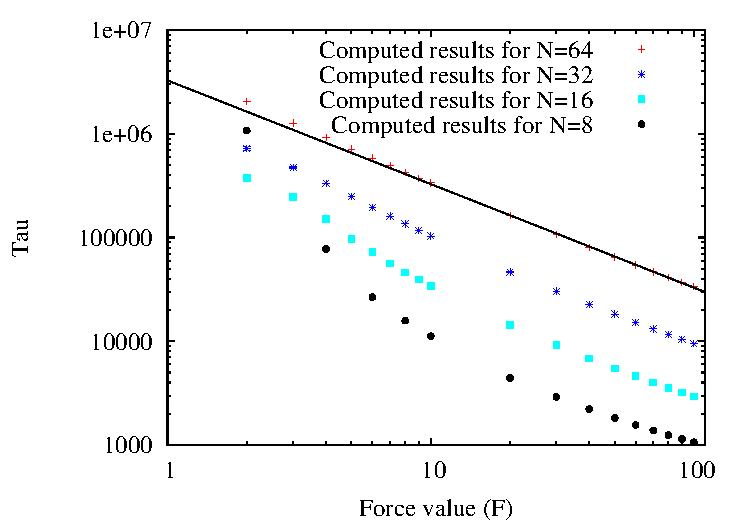
\includegraphics[width=0.48\textwidth]{translocfthinpore.pdf} 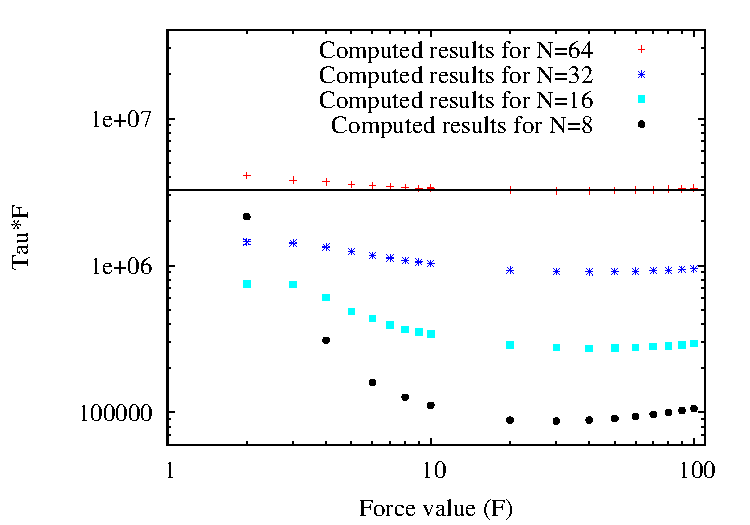
\includegraphics[width=0.48\textwidth]{translocthinpore.pdf}

\caption{Lors de la translocation à travers un nanopore étroit, la transition entre les les deux régimes observés précédemment semble se faire pour des forces plus élevées. Le frottement pourrait être caractérisé par une diminution de la force effective. La loi $\tau \propto N^{1+\nu}$ est toujours suivie. La modification de la barrière d'énergie introduit un comportement imprévu à gauche de la courbe. Le comportement anormal du cas $N=8$ à faible forces est dû a des effets de tailles finies et aux conditions de test lors des simulations.}
\label{thinpore}
\end{center}
\end{figure}

Les lois d'échelles ne semblent pas avoir été modifiées à fortes forces, si ce n'est en introduisant une force effective à cause du frottement. L'application d'une force faible sur un nanopore étroit permet de ralentir la translocation (Figure \ref{both}).

\begin{figure}[H]
\begin{center}
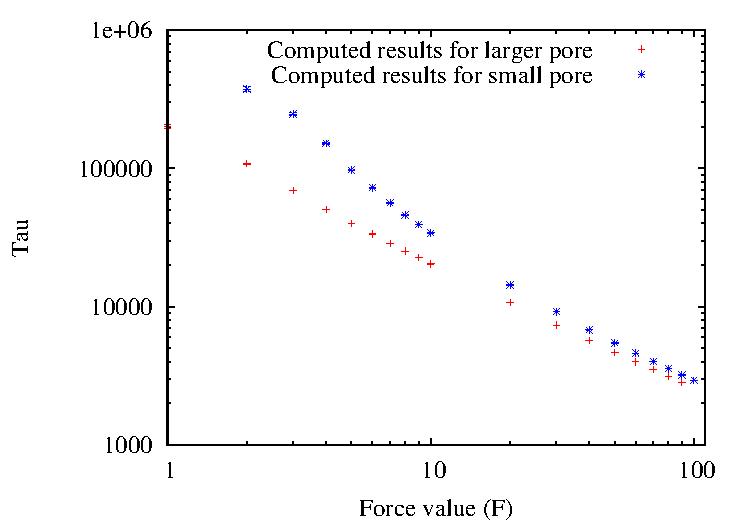
\includegraphics[width=0.45\textwidth]{translocporedifn.pdf} 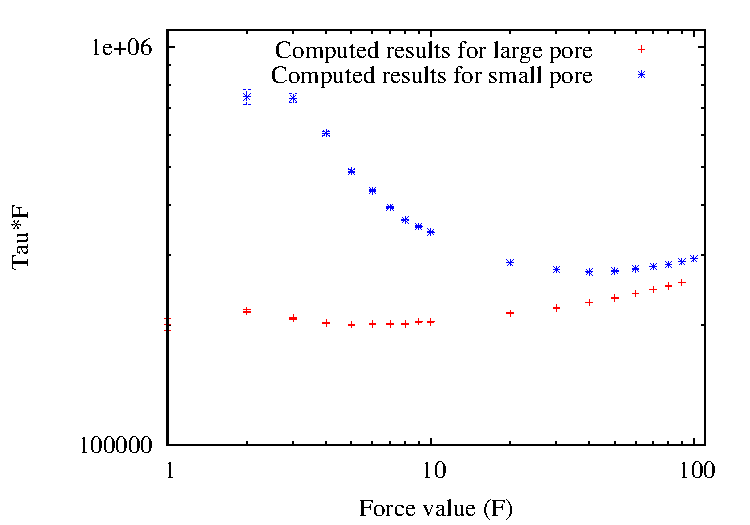
\includegraphics[width=0.45\textwidth]{translocporedif.pdf}

\caption{A forte force, l'étroitesse du pore ne modifie pas les lois d'échelles. A faible force la modification de la barrière énergétique entraine une augmentation importante du temps de translocation (ici $N=16$).}
\label{both}
\end{center}
\end{figure}

Nous allons maintenant nous intéresser à l'influence des propriétés vibrationnelles du graphène sur la translocation.

\subsubsection*{Translocation à travers un pore vibrant}

Pour les vibrations, nous avons choisi de thermaliser notre membrane a une température bien plus faible que celle du polymère ($0.005\epsilon$) afin de pouvoir observé l'échauffement du pore au cours de la translocation. Afin de conserver une trajectoire naturelle, nous avons imposé au potentiel harmonique des carbone une raideur adaptée. La Figure \ref{temperature} commente les résultats observés sur une translocation unique (en ce qui concerne les résultats ayant une signification statistique, nous obtenons des résultats surprenants montrés en annexe).
\begin{figure}[H]
\begin{center}
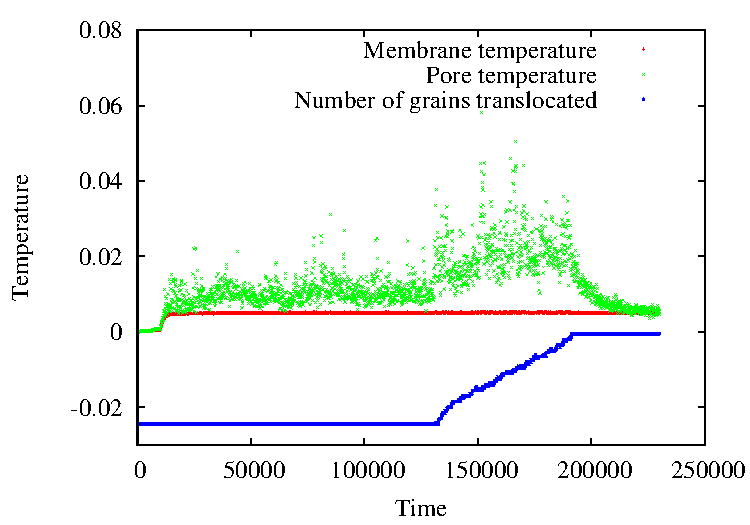
\includegraphics[width=0.49\textwidth]{tempmurmobil.pdf}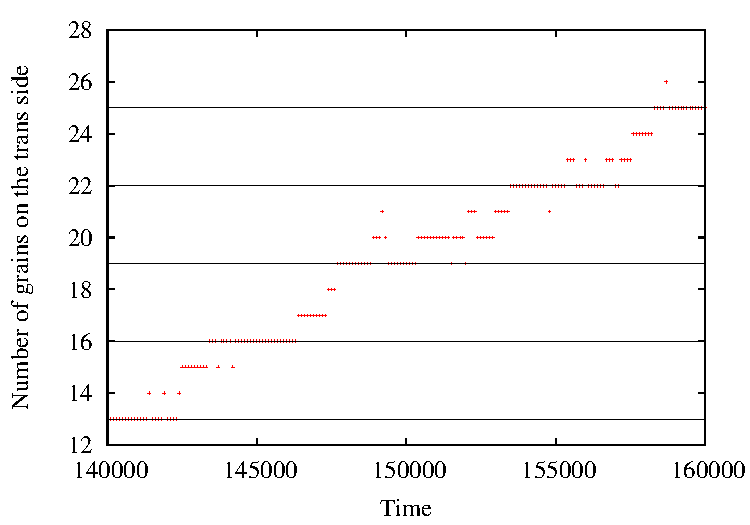
\includegraphics[width=0.49\textwidth]{murmobil.pdf}

\caption{A gauche: Evolution de la température de la membrane et du pore au cours de la thermalisation, suivie de la translocation, le nombre de grains passés du coté trans est donné de manière indicative (échelle arbitraire). Lors de la translocation, le polymère échauffe la paroi du pore, qui retourne à l'équilibre thermique une fois la translocation terminée. A droite: Illustration de la translocation ayant lieu par paliers, le gros grain latéral passant difficilement à travers le pore.}
\label{temperature}
\end{center}
\end{figure}



\bibliography{biblio}
\bibliographystyle{unsrt}



\end{document}
